% LaTeX Präsentationsvorlage (2013) der TU Graz, rev12, 2013/01/31
% !TeX encoding = UTF-8
\documentclass{beamer}
% \documentclass[aspectratio=169]{beamer}
% \usetheme{tugraz2013}
% \usetheme[notes]{tugraz2013}
\usepackage{../common/beamerthemetugraz2013}
\usepackage{color}
\usepackage{multicol}
\usepackage{bbding}
\usepackage{wasysym}
\usepackage{caption}
\usepackage{array}
% \usepackage{minted}

\usepackage{listings}
\usepackage{xcolor}

\definecolor{codegreen}{rgb}{0,0.6,0}
\definecolor{codegray}{rgb}{0.5,0.5,0.5}
\definecolor{codepurple}{rgb}{0.58,0,0.82}
\definecolor{backcolour}{rgb}{0.95,0.95,0.92}
\lstdefinestyle{mystyle}{
    backgroundcolor=\color{backcolour},   
    commentstyle=\color{codegreen},
    keywordstyle=\color{magenta},
    numberstyle=\tiny\color{codegray},
    stringstyle=\color{codepurple},
    basicstyle=\ttfamily\footnotesize,
    breakatwhitespace=false,         
    breaklines=true,                 
    captionpos=b,                    
    keepspaces=true,                 
    numbers=left,                    
    numbersep=5pt,                  
    showspaces=false,                
    showstringspaces=false,
    showtabs=false,                  
    tabsize=2
}

\lstset{style=mystyle}

\usepackage{picture}
\usepackage{rotating}
\definecolor{darkred}{rgb}{0.85,0.16,0.0}
\definecolor{darkgreen}{rgb}{0.16,0.70,0.27}

\usepackage{xcolor}

\definecolor{verylightgray}{rgb}{0.97, 0.97, 0.97}
\newcommand{\hrefu}[2]{\underline{\href{#1}{#2}}}
\newcommand{\hyperlinku}[2]{\underline{\hyperlink{#1}{#2}}}
\newcommand{\smallurl}[1]{%
  \begin{flushleft}
    \tiny\url{#1}
  \end{flushleft}
}
\newcommand{\smalltext}[1]{%
  \begin{flushleft}
    \tiny{#1}
  \end{flushleft}
}
\newcommand{\red}[1]{{\color{red} #1}}
\newcommand{\blue}[1]{{\color{blue} #1}}
\newcommand{\darkgreen}[1]{\textcolor{darkgreen}{#1}}
\newcommand{\darkred}[1]{\textcolor{darkred}{#1}}

\newcommand*{\vpointer}{\vcenter{\hbox{\scalebox{1.5}{\large\pointer}}}}

\newcommand{\be}[1]{\begin{equation} \label{#1}}
\newcommand{\ee}{\end{equation}}
\newcommand{\bea}[1]{\begin{eqnarray} \label{#1}}
\newcommand{\eea}{\end{eqnarray}}
\newcommand{\bean}{\begin{eqnarray*}}
\newcommand{\eean}{\end{eqnarray*}}

\newcommand{\non}{\nonumber\\}
\newcommand{\eq}[1]{(\ref{#1})}
\newcommand{\difp}[2]{\frac{\partial #1}{\partial #2}}
\newcommand{\br}{{\bf r}}
\newcommand{\bR}{{\bf R}}
\newcommand{\bA}{{\bf A}}
\newcommand{\bB}{{\bf B}}
\newcommand{\bE}{{\bf E}}
\newcommand{\bm}{{\bf m}}
%\renewcommand{\bm}{{\bf m}}
\newcommand{\bn}{{\bf n}}
\newcommand{\bN}{{\bf N}}
\newcommand{\bp}{{\bf p}}
\newcommand{\bP}{{\bf P}}
\newcommand{\bF}{{\bf F}}
\newcommand{\by}{{\bf y}}
\newcommand{\bz}{{\bf z}}
\newcommand{\bZ}{{\bf Z}}
\newcommand{\bV}{{\bf V}}
\newcommand{\bv}{{\bf v}}
\newcommand{\bu}{{\bf u}}
\newcommand{\bx}{{\bf x}}
\newcommand{\bX}{{\bf X}}
\newcommand{\bW}{{\bf W}}
\newcommand{\bJ}{{\bf J}}
\newcommand{\bj}{{\bf j}}
\newcommand{\bk}{{\bf k}}
\newcommand{\bTheta}{{\bf \Theta}}
\newcommand{\btheta}{{\boldsymbol\theta}}
\newcommand{\bOmega}{{\bf \Omega}}
\newcommand{\bomega}{{\boldsymbol\omega}}
\newcommand{\brho}{{\boldsymbol\rho}}
\newcommand{\rd}{{\rm d}}
\newcommand{\rJ}{{\rm J}}
\newcommand{\ph}{{\varphi}}
\newcommand{\te}{\theta}
\newcommand{\tht}{\vartheta}
\newcommand{\vpar}{v_\parallel}
\newcommand{\vparkb}{v_{\parallel k b}}
\newcommand{\vparkm}{v_{\parallel k m}}
\newcommand{\Jpar}{J_\parallel}
\newcommand{\ppar}{p_\parallel}
\newcommand{\Bpstar}{B_\parallel^*}
\newcommand{\intpi}{\int\limits_{0}^{2\pi}}
\newcommand{\summ}{\sum \limits_{m=-\infty}^\infty}
\newcommand{\tb}{\tau_b(\uv)}
\newcommand{\bh}{{\bf h}}
\newcommand{\cE}{{\cal E}}
\newcommand{\bsigma}{{\boldsymbol\sigma}}
\newcommand{\bS}{{\mathbf S}}
\newcommand{\bI}{{\mathbf I}}
\newcommand{\odtwo}[2]{\frac{\rd #1}{\rd #2}}
\newcommand{\pdone}[1]{\frac{\partial}{\partial #1}}
\newcommand{\pdtwo}[2]{\frac{\partial #1}{\partial #2}}
\newcommand{\ds}{\displaystyle} % commands


%% Titelblatt-Einstellungen
\title[]
{Python 10}
\author[E.~Wachmann]{\scriptsize Elias Wachmann
}
\date{2025} % \today für heutiges Datum verwenden
\institute[Institute of Theoretical and Computational Physics]
{
}
\instituteurl{www.tugraz.at}
% \institutelogo{kurz.pdf}
%~ \additionallogo{merged_logos}
\AtBeginSection[]{
  \begin{frame}
  \vfill
  \centering
  \begin{beamercolorbox}[sep=8pt,center,shadow=true,rounded=true]{title}
    \usebeamerfont{title}\insertsectionhead\par%
  \end{beamercolorbox}
  \vfill
  \end{frame}
}
\lstset{
    literate={Ö}{{\"O}}1
             {Ä}{{\"A}}1
             {Ü}{{\"U}}1
             {ß}{{\ss}}1
             {ü}{{\"u}}1
             {ä}{{\"a}}1
             {ö}{{\"o}}1
}

%%%%%%%%%%%%%%%%%%%%%%%%%%%%%%%%%%%%%%%%%%%%%%%%%%%%%%%%%%%%%%%%%%%%%%%%%%%%
\begin{document}
%%%%%%%%%%%%%%%%%%%%%%%%%%%%%%%%%%%%%%%%%%%%%%%%%%%%%%%%%%%%%%%%%%%%%%%%%%%%
\titleframe

%\begin{frame}
%  \frametitle{Outline}
%  \tableofcontents%[hideallsubsections] 
%  \note{
%  	Meine Präsentation ist wie folgt strukturiert \ldots
%  }
%\end{frame}

\section*{Content}

\begin{frame}
\frametitle{Content}
  \tableofcontents
\end{frame}

%%%%%%%%%%%%%%%%%%%%%%%%%%%%%%%%%%%%%%%%%%%%%%%%%%%%%%%%%%%%%%%%%%%%%%%%%%%%
\section{Uncertainties in Python}
\begin{frame}
  \frametitle{Uncertainties Package}
  The \texttt{uncertainties} package allows you to perform calculations with \hrefu{https://pythonhosted.org/uncertainties/}{\texttt{uncertainties}}
  It supports calculations with numbers that have uncertainties and automatically propagates those uncertainties through mathematical operations.\\
  \vspace{0.5cm}
  Install the package with \texttt{pip}:
  \begin{align*}
    \texttt{pip install uncertainties}
  \end{align*}
\end{frame}


\begin{frame}
  \frametitle{Basic Usage}
  To use the \texttt{uncertainties} package, you need to import the \texttt{ufloat} function, which creates numbers with uncertainties:
  \lstinputlisting[language=python, lastline=4]{examples/uncertainty1.py}
\end{frame}

\begin{frame}
  \frametitle{Propagation of Uncertainties}
  When you perform operations with these numbers, the uncertainties are automatically propagated using \hrefu{https://en.wikipedia.org/wiki/Propagation_of_uncertainty}{linear error propagation}\\
  \vspace{0.5cm}
  This is great, because you don't have to manually calculate the uncertainties of the results anymore. Just use the \texttt{nominal\_value} and \texttt{std\_dev} functions to get the result and its uncertainty:
\end{frame}

\begin{frame}
  \frametitle{Propagation of Uncertainties}
  \lstinputlisting[language=python, firstline=5, lastline=11]{examples/uncertainty1.py}
\end{frame}

\begin{frame}
  \frametitle{Mathematical Functions}
  The \texttt{uncertainties} package supports many mathematical functions, including trigonometric, exponential, and logarithmic functions:
  \lstinputlisting[language=python]{examples/uncertainty2.py}
\end{frame}


\begin{frame}
  \frametitle{Plotting with Uncertainties}
  You can also plot data with uncertainties using the \texttt{matplotlib} library:
  \lstinputlisting[language=python]{examples/uncertainty3.py}
\end{frame}

\begin{frame}
  \frametitle{Plotting with Uncertainties}
  \vspace{-5mm}
  \begin{figure}
    \centering
    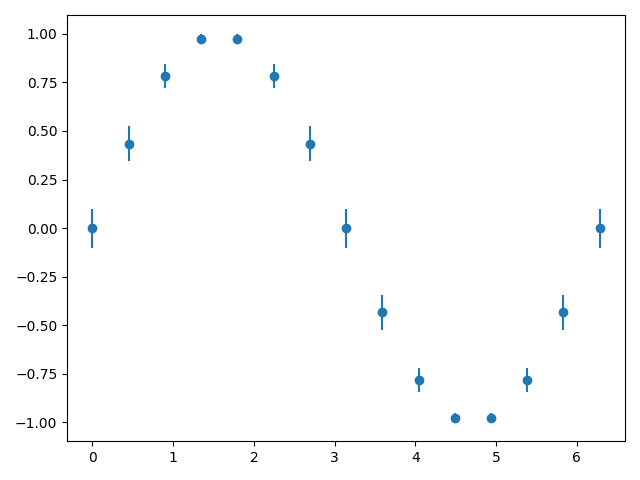
\includegraphics[width=0.75\textwidth]{examples/fig/plot.png}
  \end{figure}
\end{frame}

\begin{frame}
  \frametitle{Example: Beer-Lambert Law}
  The Beer-Lambert law relates the absorption of light to the properties of the material it passes through. It is given by:
  \begin{align*}
    I(x) = I_0 e^{-\alpha x}
  \end{align*}
  where $I(x)$ is the intensity of the light after passing through a material of thickness $x$, $I_0$ is the initial intensity, and $\alpha$ is the absorption coefficient.\\
\end{frame}

\begin{frame}
  \frametitle{Example: Beer-Lambert Law}
  Suppose we have the following measurements:
  % table with 5 measurements for different x: 
  \begin{table}[H]
    \centering
    \begin{tabular}{|c|c|c|}
      \hline
      $x$ & $I(x)$ & $\Delta I(x)$ \\
      \hline
      0.0 & 1.0 & 0.1 \\
      0.5 & 0.6 & 0.1 \\
      1.0 & 0.4 & 0.1 \\
      1.5 & 0.3 & 0.1 \\
      2.0 & 0.2 & 0.1 \\
      \hline
  \end{tabular}
  \end{table}
  and we want to determine the absorption coefficient $\alpha$ using a fit to the Beer-Lambert law.
\end{frame}
\begin{frame}
  \frametitle{Example: Beer-Lambert Law}
  \vspace{-5mm}
  \begin{figure}
    \centering
    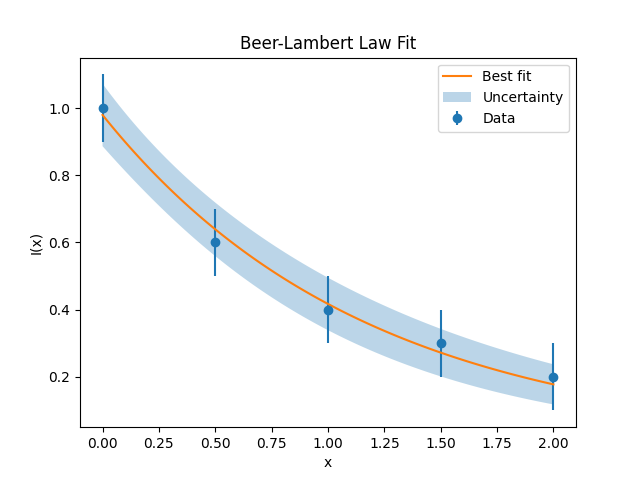
\includegraphics[width=0.75\textwidth]{examples/fig/beerLambert.png}
  \end{figure}
\end{frame}



\end{document}
%%%%%%%%%%%%%%%%%%%%%%%%%%%%%%%%%%%%%%%%%%%%%%%%%%%%%%%%%%%%%%%%%%%%%%%%%%%%

%% EOF
